\chapter{Retrosíntesis y estrategia en varias etapas}\label{ch:b2:retrosynthesis}

Se dibuja una molécula en la pizarra, y nadie sabe todavía cómo prepararla. Probar reacciones hacia delante, a partir
de lo que haya en la estantería, no lleva a ninguna parte: hay demasiadas. El químico trabaja en el otro sentido, desde la
\omterm{def:b2:retrosynthesis:analysis}{molécula objetivo} hacia la estantería, cortando un enlace cada vez sobre el papel, de modo que cada corte deshaga una reacción que
se sabe que funciona, hasta que los fragmentos sean compuestos que puedan comprarse. Este capítulo convierte las reacciones de
los capítulos anteriores en ese razonamiento hacia atrás, y se pregunta después cómo juzgar la ruta que produce.

\begin{recall}
Del \cref{ch:b2:alkene-redox} al \cref{ch:b2:wittig}: las reacciones que hay que deshacer. El volumen del primer año:
grupos protectores y acetales, reactivos de Grignard e inversión de polaridad, síntesis de Williamson,
quimioselectividad, oxidación de los alcoholes. El volumen escolar: economía atómica.
\end{recall}

\section{Pensar hacia atrás}

\begin{definition}[Análisis retrosintético]\label{def:b2:retrosynthesis:analysis}
La molécula que se quiere preparar es la \emph{molécula objetivo}\index{molecula objetivo@molécula objetivo}. El \emph{análisis retrosintético}
\index{analisis retrosintetico@análisis retrosintético} va de la molécula objetivo hacia productos de partida disponibles,
mediante etapas cada una de las cuales es la inversa de una reacción conocida; una etapa retrosintética se escribe con la
flecha doble $\Rightarrow$, que se lee ``se prepara a partir de''.
\end{definition}

\begin{definition}[Desconexión y sintones]\label{def:b2:retrosynthesis:disconnection}
Una \emph{desconexión}\index{desconexion@desconexión} es el corte imaginario de un enlace de la \omterm{def:b2:retrosynthesis:analysis}{molécula objetivo}, la
inversa de una reacción de formación de enlace. Cortar un enlace heterolíticamente da dos \emph{sintones}\index{sinton@sintón},
fragmentos cargados idealizados, uno dador (nucleófilo, a menudo negativo) y el otro aceptor
(electrófilo, a menudo positivo). Un \emph{equivalente sintético}\index{equivalente sintetico@equivalente sintético} es un
reactivo real que se comporta como un sintón: un reactivo de Grignard para el carbanión \ce{R-}, un aldehído para el
catión $\mathrm{R\overset{+}{C}H{-}OH}$.
\end{definition}

\begin{definition}[Interconversión de grupos funcionales]\label{def:b2:retrosynthesis:fgi}
Una \emph{interconversión de grupos funcionales}\index{interconversion de grupos funcionales@interconversión de grupos funcionales} (IGF) es una
etapa retrosintética que cambia un grupo funcional sin cambiar el esqueleto carbonado: un alcohol
a partir de una cetona (por reducción), una cadena alcano a partir de un alqueno (por hidrogenación), una amina a partir de una amida.
\end{definition}

\begin{omfigure}
\begin{tikzpicture}[every node/.style={align=center}]
\node (T) at (0,0) {\setchemfig{atom sep=1.7em}\chemfig{Ph-CH(-[2]OH)-CH(-[6]CH_3)-CH_3}};
\node (A) at (-4.6,-2.6) {\ce{PhCHO}\\[1pt] + \ce{(CH3)2CHMgBr}};
\node (B) at (0,-2.6) {\ce{PhMgBr}\\[1pt] + \ce{(CH3)2CHCHO}};
\node (C) at (4.6,-2.6) {\setchemfig{atom sep=1.7em}\chemfig{Ph-C(=[2]O)-CH(-[6]CH_3)-CH_3}};
\node (D) at (4.6,-5.0) {\ce{C6H6}\\[1pt] + \ce{(CH3)2CHCOCl}};
\draw[omretro] (T.south west) -- node[above left, font=\small] {a} (A.north);
\draw[omretro] (T.south) -- node[right, font=\small] {b} (B.north);
\draw[omretro] (T.south east) -- node[above right, font=\small] {IGF} (C.north);
\draw[omretro] (C.south) -- node[right, font=\small] {c} (D.north);
\end{tikzpicture}
\par\vspace{6pt}

{\small Un árbol retrosintético para el 2-metil-1-fenilpropan-1-ol. (a) y (b): las dos desconexiones del
enlace \ce{C-C} contiguo al carbono del alcohol, cada una con un aldehído y un reactivo de Grignard. IGF: el alcohol
a partir de una cetona, por reducción; (c) la cetona por \omterm{def:b2:aromatic-substitution:friedel-crafts}{acilación de Friedel--Crafts} del benceno. Cada flecha
se lee ``se prepara a partir de''.}
\end{omfigure}

El árbol muestra los hábitos del método. Se elige una \omterm{def:b2:retrosynthesis:disconnection}{desconexión} en un enlace contiguo a un grupo
funcional, porque es ahí donde las reacciones forman enlaces. Cada corte se comprueba escribiendo los \omterm{def:b2:retrosynthesis:disconnection}{sintones} y
buscándoles reactivos reales. Y rara vez hay una sola respuesta: el árbol se ramifica, y las ramas se
juzgan al final (\cref{sec:b2:retrosynthesis:judging}).

\begin{omfigure}
\begin{center}
\small
\renewcommand{\arraystretch}{1.25}
\begin{tabular}{lll}
\hline
\omterm{def:b2:retrosynthesis:disconnection}{Sintón} & Tipo & \omterm{def:b2:retrosynthesis:disconnection}{Equivalente sintético} \\
\hline
\ce{R-} (alquilo, arilo) & dador & \ce{RMgBr}, \ce{RLi}, \ce{R2CuLi} (conjugada) \\
$\mathrm{^-CH_2COR}$ & dador & el \omterm{def:b2:enolates-aldol:enolate}{enolato} de \ce{CH3COR}, o el 3-oxobutanoato de etilo \\
$\mathrm{^-C{\equiv}N}$ & dador & \ce{NaCN} \\
$\mathrm{R\overset{+}{C}H{-}OH}$ & aceptor & el aldehído \ce{RCHO} \\
$\mathrm{R\overset{+}{C}{=}O}$ & aceptor & el \omterm{def:b2:acyl-substitution:derivative}{cloruro de acilo} \ce{RCOCl}, un éster \\
\ce{R+} (primario) & aceptor & el haluro \ce{RBr} (sustitución bimolecular) \\
$\mathrm{^+CH_2CH_2COR}$ & aceptor & la enona \ce{CH2=CHCOR} (\omterm{def:b2:conjugate-additions:addition-modes}{adición conjugada}) \\
\hline
\end{tabular}
\end{center}

{\small \omterm{def:b2:retrosynthesis:disconnection}{Sintones} habituales y sus \omterm{def:b2:retrosynthesis:disconnection}{equivalentes sintéticos}. Los \omterm{def:b2:retrosynthesis:disconnection}{sintones} dadores son carbaniones, y los
\omterm{def:b2:retrosynthesis:disconnection}{sintones} aceptores, carbocationes; los reactivos reales tienen la misma polaridad sin la carga completa.}
\end{omfigure}

\section{Desconexiones de un grupo}

Una \omterm{def:b2:retrosynthesis:disconnection}{desconexión} de un grupo corta un enlace contiguo a un único grupo funcional. Para un enlace \ce{C-O} o \ce{C-N}
de un éter, un éster o una amina, el corte pasa entre el carbono y el heteroátomo: el heteroátomo es
el dador, y el carbono, el aceptor (una síntesis de Williamson, una \omterm{def:b2:acyl-substitution:esterification}{esterificación}, una formación de amida).
Para un enlace \ce{C-C}, el grupo funcional fija la polaridad de los \omterm{def:b2:retrosynthesis:disconnection}{sintones}: junto a un carbono de alcohol,
el carbono del alcohol es el aceptor (un aldehído o una cetona) y el otro carbono, el dador (un
organometálico); junto a un carbonilo, el carbono $\alpha$ es el dador (un \omterm{def:b2:enolates-aldol:enolate}{enolato}).

La mayoría de estas reacciones necesitan el nivel de oxidación adecuado en el lugar adecuado, de modo que las IGF entre niveles
de oxidación son las etapas más frecuentes de una ruta: alqueno, alcohol, aldehído o cetona, ácido. Una de ellas quedó
pendiente en el volumen del primer año: detener la oxidación de un alcohol primario en el aldehído.

\begin{proposition}[Oxidaciones suaves]\label{prop:b2:retrosynthesis:mild-oxidation}
Un alcohol primario se oxida al aldehído, sin seguir hasta el ácido, con un oxidante usado en un
disolvente orgánico anhidro: el clorocromato de piridinio en diclorometano, la oxidación de Swern (dimetil
sulfóxido activado con cloruro de oxalilo, y luego trietilamina, a baja temperatura) o el peryodinano de
Dess--Martin. En agua, el cromo(VI) o el permanganato lo oxidan al ácido carboxílico.
\end{proposition}

\begin{proof}[Argumento]
Estos oxidantes arrancan el hidrógeno del enlace \ce{C-H} del carbono que lleva un \ce{OH}. El aldehído
formado no tiene ese grupo. En agua, sin embargo, un aldehído está en equilibrio con su hidrato
\ce{RCH(OH)2}, que de nuevo tiene un \ce{OH} sobre un carbono que lleva un hidrógeno: el hidrato se oxida
como un alcohol, hasta el ácido. Sin agua no se forma hidrato, y la oxidación se detiene en el
aldehído.
\end{proof}

\section{Desconexiones de dos grupos}

Cuando la \omterm{def:b2:retrosynthesis:analysis}{molécula objetivo} tiene dos grupos funcionales, la mejor \omterm{def:b2:retrosynthesis:disconnection}{desconexión} suele aprovechar ambos: el enlace se corta
de modo que un grupo dirige al dador y el otro al aceptor. La distancia entre los grupos,
contada en carbonos de un carbono funcionalizado al otro, ambos inclusive, indica qué reacción usar.

\begin{proposition}[Disposiciones y sus reacciones]\label{prop:b2:retrosynthesis:patterns}
Las relaciones entre dos grupos se corresponden con las reacciones de los capítulos anteriores como sigue. Las
relaciones impares (1,3 y 1,5) concuerdan con las polaridades naturales de la química de los carbonilos; las pares (1,4
y 1,6) no, y requieren una inversión de polaridad o la ruptura de un anillo.
\end{proposition}


\begin{proof}[Argumento]
En la química de los carbonilos el carbono carbonílico es un aceptor y el carbono $\alpha$ un dador, y una enona
añade un aceptor en su carbono $\beta$. Un \omterm{def:b2:enolates-aldol:enolate}{enolato} (dador en $\alpha$) sobre un carbonilo (aceptor en el
carbono carbonílico) une los carbonos 1 y 2 de una disposición 1,3: \omterm{def:b2:enolates-aldol:aldol}{aldólica} y Claisen. Un \omterm{def:b2:enolates-aldol:enolate}{enolato} sobre el carbono $\beta$
de una enona construye una disposición 1,5: Michael, y luego Robinson. Para una disposición 1,4, el corte deja un
carbono $\alpha$ como aceptor; ningún reactivo carbonílico ordinario ofrece esa polaridad, pero una $\alpha$-bromo
cetona sí, ya que el bromuro es un grupo saliente en ese carbono. Un compuesto 1,6-dicarbonílico es un ciclohexeno abierto
por \omterm{def:b2:alkene-redox:cleavage}{ozonólisis} (\cref{prop:b2:alkene-redox:ozonolysis}), y el ciclohexeno se prepara por una \omterm{def:b2:frontier-orbitals:diels-alder}{reacción de
Diels--Alder} (\cref{def:b2:frontier-orbitals:diels-alder}).
\end{proof}

\begin{omfigure}
\begin{center}
\small
\renewcommand{\arraystretch}{1.25}
\begin{tabular}{lll}
\hline
Disposición & \omterm{def:b2:retrosynthesis:disconnection}{Desconexión} & Reacción \\
\hline
carbonilo $\beta$-hidroxilado (1,3) & enlace $\alpha$--$\beta$ & \omterm{def:b2:enolates-aldol:aldol}{adición aldólica} \\
carbonilo $\alpha,\beta$-insaturado & \ce{C=C} & \omterm{def:b2:enolates-aldol:aldol}{condensación aldólica} \\
1,3-dicarbonilo & C(O)--C$\alpha$ & \omterm{def:b2:enolates-aldol:claisen}{condensación de Claisen} \\
1,5-dicarbonilo & C$\alpha$--C$\beta$ del aceptor & \omterm{def:b2:conjugate-additions:michael}{adición de Michael} \\
ciclohex-2-en-1-ona & \ce{C=C} del anillo + Michael & \omterm{def:b2:conjugate-additions:robinson}{anulación de Robinson} \\
ciclohexeno & dos enlaces \ce{C-C} del anillo & \omterm{def:b2:frontier-orbitals:diels-alder}{reacción de Diels--Alder} \\
alqueno en posición definida & \ce{C=C} & \omterm{def:b2:wittig:wittig}{reacción de Wittig} o HWE \\
1,4-dicarbonilo & \ce{C-C} central & \omterm{def:b2:enolates-aldol:enolate}{enolato} + $\alpha$-halo cetona \\
1,6-dicarbonilo & reunir los extremos & \omterm{def:b2:alkene-redox:cleavage}{ruptura oxidante} de un ciclohexeno \\
\hline
\end{tabular}
\end{center}

{\small Las desconexiones de dos grupos. Las seis primeras usan la polaridad normal: un \omterm{def:b2:enolates-aldol:enolate}{enolato} (dador) sobre un
carbonilo o una enona (aceptor). La disposición 1,4 necesita que un carbono en $\alpha$ de un carbonilo sea el
aceptor, al revés de su papel habitual, cosa que proporciona una $\alpha$-halo cetona.}
\end{omfigure}

\begin{method}[Un análisis retrosintético]\label{met:b2:retrosynthesis:retrosynthesis}
\begin{enumerate}
  \item Enumérense los grupos funcionales de la \omterm{def:b2:retrosynthesis:analysis}{molécula objetivo} y sus relaciones (1,2; 1,3; \dots).
  \item Considérense las IGF que darían una disposición con una buena \omterm{def:b2:retrosynthesis:disconnection}{desconexión} (un alcohol a partir de una cetona, una
        cadena alcano a partir de un alqueno).
  \item Elíjanse enlaces estratégicos: contiguos a un grupo funcional, cerca del centro de la molécula, en un
        punto de ramificación o uniendo un anillo a una cadena, de modo que los fragmentos sean de tamaño parecido.
  \item Escríbanse los \omterm{def:b2:retrosynthesis:disconnection}{sintones} y luego sus \omterm{def:b2:retrosynthesis:disconnection}{equivalentes sintéticos}; descártese un corte sin reactivo real.
  \item Compruébese la quimioselectividad: ¿qué otro grupo reaccionaría con cada reactivo? Planifíquese una protección
        o cámbiese el orden de las etapas.
  \item Repítase con cada fragmento hasta que todos estén disponibles; escríbase después la ruta hacia delante, con reactivos y
        condiciones.
\end{enumerate}
\end{method}

\section{Grupos protectores en una ruta}

Una ruta necesita a menudo un reactivo que atacaría un segundo grupo de la molécula. El volumen del primer año
protegía aldehídos y cetonas como acetales. Una ruta elige entre varios grupos protectores, cada uno
eliminado en sus propias condiciones: acetales (eliminados con ácido acuoso), éteres sililados de los alcoholes (eliminados con el
ion fluoruro), éteres bencílicos (eliminados por hidrogenólisis sobre paladio), carbamatos de las aminas como
el grupo \textit{terc}-butoxicarbonilo (eliminado con ácido) y ésteres (eliminados con base).

\begin{definition}[Protección ortogonal]\label{def:b2:retrosynthesis:orthogonal}
Un conjunto de \emph{grupos protectores ortogonales}\index{grupos protectores ortogonales} es un conjunto de grupos
protectores cada uno de los cuales puede eliminarse en condiciones que dejan intactos todos los demás, de modo que las funciones que enmascaran
pueden liberarse de una en una, en cualquier orden.
\end{definition}

\begin{method}[Proteger en una ruta]\label{met:b2:retrosynthesis:protect-in-route}
\begin{enumerate}
  \item Para cada etapa, enumérense los grupos que el reactivo atacaría además del deseado.
  \item Inténtese primero evitar la protección: cámbiese el orden de las etapas, o úsese un reactivo más selectivo
        (un borohidruro en lugar de un hidruro para una cetona junto a un éster).
  \item Si no, elíjase un grupo estable en todas las etapas hasta su eliminación, y eliminable en condiciones que la
        molécula tolere.
  \item Con varios grupos que liberar por separado, elíjase un conjunto ortogonal.
  \item Búsquese una etapa que elimine un grupo sin coste: una hidrogenación prevista de todos modos elimina también un
        éter bencílico.
  \item Cuéntese: cada protección cuesta dos etapas y sus rendimientos.
\end{enumerate}
\end{method}

\section{Juzgar una ruta}\label{sec:b2:retrosynthesis:judging}

\begin{proposition}[Rendimiento global]\label{prop:b2:retrosynthesis:overall-yield}
El rendimiento global de una secuencia lineal de etapas es el producto de los rendimientos de las etapas:
$\rho = \rho_1 \rho_2 \cdots \rho_n$. Con $n$ etapas de igual rendimiento $\rho_1$, $\rho = \rho_1^{\,n}$.
\end{proposition}

\begin{proof}
La etapa $k$ convierte la cantidad $n_{k-1}$ de su producto de partida en $n_k = \rho_k\, n_{k-1}$ de producto
(rendimientos referidos a las cantidades del intermedio, con todos los demás reactivos en cantidad suficiente). Por inducción,
$n_n = \rho_n \rho_{n-1} \cdots \rho_1\, n_0$, y el rendimiento global $n_n/n_0$ es el producto.
\end{proof}

\begin{omfigure}
\begin{tikzpicture}
\begin{axis}[width=0.75\linewidth, height=5.4cm, xmin=0, xmax=20, ymin=0, ymax=100,
  xlabel={número de etapas $n$}, ylabel={rendimiento global (\%)}, label style={font=\small},
  tick label style={font=\scriptsize}, xtick={0,5,10,15,20}, grid=major, grid style={black!12},
  legend style={font=\scriptsize, at={(0.98,0.98)}, anchor=north east}, legend cell align=left]
\addplot[omDef, thick] table[x=n, y=r95] {figdata/out/bachelor-2-overall-yield.dat};
\addplot[omThm, thick] table[x=n, y=r90] {figdata/out/bachelor-2-overall-yield.dat};
\addplot[omMeth, thick] table[x=n, y=r80] {figdata/out/bachelor-2-overall-yield.dat};
\addplot[black!60, thick, dashed] table[x=n, y=r70] {figdata/out/bachelor-2-overall-yield.dat};
\legend{95~\% por etapa, 90~\% por etapa, 80~\% por etapa, 70~\% por etapa}
\end{axis}
\end{tikzpicture}
\par\vspace{4pt}

{\small Rendimiento global de una ruta lineal en función de su número de etapas, para cuatro rendimientos por etapa
(\cref{prop:b2:retrosynthesis:overall-yield}). Diez etapas al 90~\% cada una conservan el 35~\% del material; diez
etapas al 70~\%, menos del 3~\%.}
% figdata: bachelor-2/overall-yield.py
\end{omfigure}

La regla del producto explica por qué ganan las rutas cortas, por qué una protección (dos etapas más) nunca es gratuita, y por qué
los químicos prefieren construir dos mitades por separado y unirlas tarde: la ruta larga se recorre entonces en dos
ramas más cortas, y las pérdidas de una rama no se multiplican por las de la otra. Además del rendimiento y de la
longitud, una ruta se juzga por su \omterm{def:b2:continuous-reactors:selectivity}{selectividad} (cada etapa debería dar un solo producto), por el coste y el peligro
de sus reactivos, por los residuos que genera (la economía atómica de cada etapa y los disolventes de las
purificaciones) y por la facilidad con que cada etapa se lleva a mayor escala.

\begin{history}[El razonamiento hacia atrás, hecho explícito]
\begin{minipage}[t]{0.2\linewidth}
\vspace{0pt}
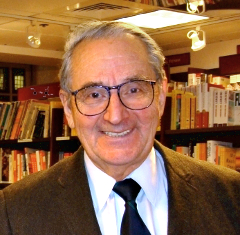
\includegraphics[width=\linewidth]{images/book3/corey.jpg}
\end{minipage}\hfill
\begin{minipage}[t]{0.76\linewidth}
\vspace{0pt}
Los químicos siempre habían razonado hacia atrás desde sus \omterm{def:b2:retrosynthesis:analysis}{moléculas objetivo}, pero Elias James Corey, a partir de los años sesenta,
convirtió el hábito en reglas explícitas: la \omterm{def:b2:retrosynthesis:disconnection}{desconexión}, el \omterm{def:b2:retrosynthesis:disconnection}{sintón}, la flecha retrosintética, e
incluso programas informáticos que las aplicaban. Recibió el Premio Nobel de Química de 1990 por la teoría
y la metodología de la síntesis orgánica. (Fotografía: de Trvthchem, CC0, Wikimedia Commons.)
\end{minipage}
\end{history}

\begin{safety}{\ghs[5mm]{GHS02}\,\ghs[5mm]{GHS03}\,\ghs[5mm]{GHS05}\,\ghs[5mm]{GHS06}\,\ghs[5mm]{GHS07}\,\ghs[5mm]{GHS08}}
El cloruro de oxalilo es corrosivo y tóxico y reacciona con el agua, desprendiendo cloruro de hidrógeno; la oxidación de Swern
desprende monóxido de carbono y sulfuro de dimetilo, maloliente, por lo que se lleva a cabo en una vitrina de gases.
El peryodinano de Dess--Martin es un oxidante y no debe calentarse. Los reactivos de cromo(VI) se evitan hoy
siempre que existe una alternativa.
% ledger: ghs:oxalyl-chloride, ghs:DMSO, ghs:DMP
\end{safety}

\section{Ejercicios}

\begin{exercise}[$\star$]\label{exo:b2:retrosynthesis:1}
Desconéctese cada alcohol en un compuesto carbonílico y un reactivo de Grignard (dense todas las posibilidades):
2-fenilpropan-2-ol, pentan-3-ol, 1-ciclohexiletanol, 2-metilbutan-2-ol, 1-feniletanol.
\end{exercise}

\begin{exercise}[$\star$]\label{exo:b2:retrosynthesis:2}
Para la \omterm{def:b2:retrosynthesis:disconnection}{desconexión} del 1-feniletanol en el enlace \ce{C-C}, nómbrense los dos \omterm{def:b2:retrosynthesis:disconnection}{sintones}, dígase cuál es el
dador, y dese un \omterm{def:b2:retrosynthesis:disconnection}{equivalente sintético} de cada uno.
\end{exercise}

\begin{exercise}[$\star$]\label{exo:b2:retrosynthesis:3}
Una ruta de cinco etapas tiene rendimientos por etapa del 90, 85, 80, 95 y 70~\%. Calcúlese su rendimiento global.
\end{exercise}

\begin{exercise}[$\star$]\label{exo:b2:retrosynthesis:4}
El 4-oxopentanoato de etilo debe convertirse en 5-hidroxipentan-2-ona. Planifíquese la ruta con un grupo
protector, y dígase por qué es necesario.
\end{exercise}

\begin{exercise}[$\star\star$]\label{exo:b2:retrosynthesis:5}
Propóngase una retrosíntesis del butano-1,3-diol a partir de compuestos de dos carbonos como máximo, con una IGF y una
\omterm{def:b2:retrosynthesis:disconnection}{desconexión} de dos grupos.
\end{exercise}

\begin{exercise}[$\star\star$]\label{exo:b2:retrosynthesis:6}
Desconéctese la 1-(ciclohex-3-en-1-il)etan-1-ona mediante una \omterm{def:b2:frontier-orbitals:diels-alder}{reacción de Diels--Alder}.
\end{exercise}

\begin{exercise}[$\star\star$]\label{exo:b2:retrosynthesis:7}
Desconéctese la 4,4-dimetilciclohex-2-en-1-ona mediante una \omterm{def:b2:conjugate-additions:robinson}{anulación de Robinson}.
\end{exercise}

\begin{exercise}[$\star\star$]\label{exo:b2:retrosynthesis:8}
La 1-fenilbutan-1-ona puede prepararse en una etapa por una \omterm{def:b2:aromatic-substitution:friedel-crafts}{acilación de Friedel--Crafts}, o en dos a partir del benzaldehído.
Escríbanse ambas rutas y compárense.
\end{exercise}

\begin{exercise}[$\star\star$]\label{exo:b2:retrosynthesis:9}
Se quiere obtener hexanal a partir del hexan-1-ol. ¿Qué reactivos lo dan, y cuál daría en cambio ácido hexanoico?
Explíquese.
\end{exercise}

\begin{exercise}[$\star\star\star$]\label{exo:b2:retrosynthesis:10}
En el 4-aminobutan-1-ol, la amina debe reaccionar primero con un \omterm{def:b2:acyl-substitution:derivative}{cloruro de acilo} en una etapa, y el alcohol
después con otro. Propóngase un par ortogonal de grupos protectores y la secuencia.
\end{exercise}

\begin{exercise}[$\star\star\star$]\label{exo:b2:retrosynthesis:11}
Propóngase una síntesis de la hexano-2,5-diona, un compuesto 1,4-dicarbonílico, a partir del 3-oxobutanoato de etilo.
\end{exercise}

\begin{exercise}[$\star\star\star$]\label{exo:b2:retrosynthesis:12}
La 6-metilhept-5-en-2-ona, \ce{(CH3)2C=CHCH2CH2COCH3}, es un intermedio de perfumería. Propóngase un plan completo
a partir del 3-oxobutanoato de etilo y un haluro: retrosíntesis, ruta hacia delante y la etapa que elimina el
éster.
\end{exercise}

\section{Problema: la cetona de frambuesa}

\begin{problem}[{Problema de fin de semana --- la retrosíntesis de un aroma, el fenol y si hay que
protegerlo, una alternativa con paladio, y el juicio de las rutas}]
\label{pb:b2:retrosynthesis:1}
La cetona de frambuesa, 4-(4-hidroxifenil)butan-2-ona, se encuentra en las frambuesas y en otras frutas y se usa
como aromatizante y en perfumería. Datos de ejercicio: rendimientos por etapa de la ruta \omterm{def:b2:enolates-aldol:aldol}{aldólica}, 85~\% (condensación)
y 92~\% (hidrogenación). Masas molares (\unit{g/mol}): C 12.011, H 1.008, O 15.999, N 14.007,
I 126.90. El $\mathrm pK_a$ del fenol es 9.99.
% ledger: use:raspberry-ketone, aw:C, aw:H, aw:O, aw:N, aw:I, pka:phenol, ghs:raspberry-ketone, ghs:4-iodophenol, ghs:MVK

\medskip
\noindent\textbf{Parte I --- Retrosíntesis.}
\begin{enumerate}
  \item Dibújese la \omterm{def:b2:retrosynthesis:analysis}{molécula objetivo} y nómbrense sus grupos funcionales.
  \item ¿Qué IGF convierte la unidad \ce{ArCH2CH2CO} en una disposición con una \omterm{def:b2:retrosynthesis:disconnection}{desconexión} conocida?
  \item Escríbase la cetona insaturada obtenida, con su geometría.
  \item ¿Qué disposición de dos grupos contiene, y qué reacción la produce?
  \item Nómbrense los dos productos de partida.
  \item ¿Por qué esta \omterm{def:b2:enolates-aldol:aldol}{aldólica} cruzada da un producto principal?
  \item Escríbase la ruta hacia delante en dos etapas, con las condiciones.
\end{enumerate}

\medskip
\noindent\textbf{Parte II --- El fenol.}
\begin{enumerate}[resume]
  \item En hidróxido de sodio acuoso, ¿en qué forma está presente el 4-hidroxibenzaldehído? Úsese el
        $\mathrm pK_a$.
  \item ¿Cómo cambia esa forma la electrofilia del aldehído?
  \item Si el fenol estuviera protegido, ¿qué grupo eliminaría sin coste la segunda etapa? Explíquese.
  \item Cuéntense las etapas de la ruta con esa protección.
  \item ¿Corre peligro el anillo bencénico en la hidrogenación?
  \item ¿Proteger o no? Conclúyase.
\end{enumerate}

\medskip
\noindent\textbf{Parte III --- Una alternativa con paladio.}
\begin{enumerate}[resume]
  \item Desconéctese la cetona insaturada en el enlace entre el anillo y la cadena: ¿qué compañeros de
        Heck?
  \item Escríbase la reacción de Heck con trietilamina como base.
  \item ¿En qué carbono de la but-3-en-2-ona acaba el grupo arilo, y por qué?
  \item Nómbrense las etapas del \omterm{def:b2:catalytic-cycles:cycle}{ciclo catalítico}.
  \item Calcúlese la economía atómica de la etapa de Heck, contando la trietilamina.
  \item Calcúlese la economía atómica de la \omterm{def:b2:enolates-aldol:aldol}{condensación aldólica}.
\end{enumerate}

\medskip
\noindent\textbf{Parte IV --- Juzgar las rutas.}
\begin{enumerate}[resume]
  \item ¿Cuál es la economía atómica de la hidrogenación?
  \item Calcúlese la economía atómica global de la ruta \omterm{def:b2:enolates-aldol:aldol}{aldólica}.
  \item ¿Qué doble enlace reduce la hidrogenación, y por qué sobrevive la cetona?
  \item Compárense los reactivos de las dos rutas en cuanto a coste y peligro.
  \item ¿Qué ruta se elegiría?
  \item ¿Qué supondría para el rendimiento global una tercera etapa al 90~\%?
  \item Indíquese el rendimiento global de la ruta \omterm{def:b2:enolates-aldol:aldol}{aldólica} en dos etapas.
\end{enumerate}
\end{problem}
